% Copyright © 2018, Loïc Grobol <loic.grobol@gmail.com>
% This document is available under the terms of the Creative Commons Attribution 4.0 International License (CC BY 4.0) (https://creativecommons.org/licenses/by/4.0/)

\RequirePackage{xparse}
\RequirePackage{shellesc}
% Settings
\NewDocumentCommand\myname{}{Loïc Grobol}
\NewDocumentCommand\mylab{}{Lattice / ALMAnaCH}
\NewDocumentCommand\pdftitle{}{Introduction à la fouille de textes}
\NewDocumentCommand\mymail{}{loic.grobol@gmail.com}
\NewDocumentCommand\titlepagetitle{}{\pdftitle}
\NewDocumentCommand\docdate{}{2019-01-21}
\NewDocumentCommand\conference{}{M1 Plurital}

\documentclass[hyperref={unicode}, xcolor={svgnames}, french]{beamer}
\usetheme[sectionpage=progressbar,
          subsectionpage=progressbar,
          progressbar=frametitle]{metropolis}
    \definecolor{accent}{RGB}{51, 34, 136}
    \setbeamercolor{alerted text}{fg=accent}
    \makeatletter
        \setlength{\metropolis@progressinheadfoot@linewidth}{1pt}
    \makeatother
    % FIXME: not pretty and footnotes are still too big
    \let\footnoterule\relax  % No footnote rule, push down footnote

% TODO: update these to the last version
% 9-Highlights colour palette from [Paul Tol's technical note](https://personal.sron.nl/~pault/data/colourschemes.pdf)
\definecolor{highlight0}{RGB}{51, 34, 136}    % Deep blue
\definecolor{highlight1}{RGB}{136, 204, 238}  % Clear blue
\definecolor{highlight2}{RGB}{68, 170, 153}   % Teal
\definecolor{highlight3}{RGB}{17, 119, 51}    % Forest green
\definecolor{highlight4}{RGB}{153, 153, 51}   % Khaki
\definecolor{highlight5}{RGB}{221, 204, 119}  % Beige
\definecolor{highlight6}{RGB}{204, 102, 119}  % Pink
\definecolor{highlight7}{RGB}{136, 34, 85}    % Purple
\definecolor{highlight8}{RGB}{170, 68, 153}   % Violet

% Alternative navy blue for ⩽4 palettes
\definecolor{highlighta}{RGB}{68, 118, 170}  % Navy blue

% Use non-standard fonts
\usefonttheme{professionalfonts}
\setsansfont[BoldFont={Fira Sans SemiBold}, ItalicFont={Fira Sans Book Italic}]{Fira Sans Book}
\setmonofont[Scale=0.9]{Fira Mono}

% Fix missing glyphs in Fira by delegating to polyglossia/babel
\usepackage{newunicodechar}
\newunicodechar{ }{~}   % U+202F NARROW NO-BREAK SPACE
\newunicodechar{ }{ }  % U+2009 THIN SPACE

% Notes on left screen
% \usepackage{pgfpages}
% \setbeameroption{show notes on second screen=left}


\usepackage[french, english]{babel}
\usepackage{amsfonts,amssymb}
\usepackage{amsmath,amsthm}
\usepackage{mathtools}	% AMS Maths service pack
	\newtagform{brackets}{[}{]}	% Pour des lignes d'équation numérotées entre crochets
	\mathtoolsset{showonlyrefs, showmanualtags, mathic}	% affiche les tags manuels (\tag et \tag*) et corrige le kerning des maths inline dans un bloc italique voir la doc de mathtools
	\usetagform{brackets}	% Utilise le style de tags défini plus haut
\usepackage{lualatex-math}

\usepackage[math-style=french]{unicode-math}
	\setmathfont{Libertinus Math}
\usepackage{newunicodechar}
	\newunicodechar{√}{\sqrt}
\usepackage{mleftright}


\usepackage{tabu}
\usepackage{booktabs}
\usepackage{siunitx}
\usepackage{multicol}
\usepackage{ccicons}
\usepackage{bookmark}
\usepackage{caption}
    \captionsetup{skip=1ex}
\usepackage[iso]{datetime}

\usepackage{csquotes}
\usepackage{tikz}
	\NewDocumentCommand{\textnode}{O{}mm}{\tikz[remember picture, baseline=(#2.base), inner sep=0pt]{\node[#1] (#2) {#3};}}
    \NewDocumentCommand{\mathnode}{O{}mm}{\tikz[remember picture, baseline=(#2.base), inner sep = 0pt]{\node[#1] (#2) {$\displaystyle #3$};}}
	\tikzset{
		alt/.code args={<#1>#2#3}{%
		\alt<#1>{\pgfkeysalso{#2}}{\pgfkeysalso{#3}} % \pgfkeysalso doesn't change the path
		},
        invisible/.style={opacity=0, fill opacity=0},
		visible on/.style={alt={<#1>{}{invisible}}}
	}
    \usepackage{forest}
    \usepackage{tkz-graph}
    \usepackage[beamer, markings]{hf-tikz}
    \usepackage{tikz-3dplot}
    \usepackage{pgfplots}
        % Due to pgfplots meddling with pgfkeys, we have to redefine alt here.
        \pgfplotsset{
    		alt/.code args={<#1>#2#3}{%
    		\alt<#1>{\pgfkeysalso{#2}}{\pgfkeysalso{#3}} % \pgfkeysalso doesn't change the path
    		},
    	}
        \pgfplotsset{compat=1.15}
        \pgfplotsset{colormap={SRON}{rgb255=(61,82,161) rgb255=(255,250,210) rgb255=(174,28,62)}}

    \usetikzlibrary{matrix}
    \usetikzlibrary{shapes, shapes.geometric}
    \usetikzlibrary{decorations.pathreplacing}
	\usetikzlibrary{positioning, calc, intersections}
    \usetikzlibrary{fit}
    \usetikzlibrary{backgrounds}

    % Do evil things with soft path
    % From <https://tex.stackexchange.com/a/301364/8547>
    % Græcum est, non legitur
    \makeatletter
        \def\@appendnamedsoftpath#1{%
            \pgfsyssoftpath@getcurrentpath\@temppatha
            \expandafter\let\expandafter\@temppathb\csname tikz@intersect@path@name@#1\endcsname
            \expandafter\expandafter\expandafter\def\expandafter\expandafter\expandafter\@temppatha\expandafter\expandafter\expandafter{\expandafter\@temppatha\@temppathb}%
            \pgfsyssoftpath@setcurrentpath\@temppatha
        }
        \def\@appendnamedpathforactions#1{%
            \pgfsyssoftpath@getcurrentpath\@temppatha
            \expandafter\let\expandafter\@temppathb\csname tikz@intersect@path@name@#1\endcsname
            \expandafter\def\expandafter\@temppatha\expandafter{\csname @temppatha\expandafter\endcsname\@temppathb}%\usepackage{tikz-3dplot}

            \let\tikz@actions@path\@temppatha
        }

        \tikzset{
            use path for main/.code={%
                \tikz@addmode{%
                    \expandafter\pgfsyssoftpath@setcurrentpath\csname tikz@intersect@path@name@#1\endcsname
                }%
            },
            append path for main/.code={%
                \tikz@addmode{%
                    \@appendnamedsoftpath{#1}%
                }%
            },
            use path for actions/.code={%
                \expandafter\def\expandafter\tikz@preactions\expandafter{\tikz@preactions\expandafter\let\expandafter\tikz@actions@path\csname tikz@intersect@path@name@#1\endcsname}%
            },
            append path for actions/.code={%
                \expandafter\def\expandafter\tikz@preactions\expandafter{\tikz@preactions
                \@appendnamedpathforactions{#1}}%
            },
            use path/.style={%
                use path for main=#1,
                use path for actions=#1,
            },
            append path/.style={%
                append path for main=#1,
                append path for actions=#1
            }
        }
    \makeatother

    % TikZ externalisation
    \usetikzlibrary{external}
    % Create the `tikzpics/` folder if it does not exist
    \ShellEscape{mkdir -p tikzpics}
    % Only externalise pictures on demand (to avoid messing up with metropolis theme)
    \tikzset{
        external/export=false,
        external/prefix=tikzpics/
    }
    \tikzexternalize

\usepackage{minted}
	\usemintedstyle{lovelace}
	\setminted{autogobble, tabsize=2}

\usepackage[style=authoryear, block=ragged, doi=false, isbn=false]{biblatex}
    \AtEveryBibitem{
        \ifentrytype{online}
        {} {
            \iffieldequalstr{howpublished}{online}
            {
                \clearfield{howpublished}
            } {
                \clearfield{urlyear}\clearfield{urlmonth}\clearfield{urlday}
            }
        }
    }

	\addbibresource{biblio.bib}

% Compact bibliography style
\setbeamertemplate{bibliography item}[text]

\AtEveryBibitem{
    \clearfield{series}
    \clearfield{pages}
    \clearlist{publisher}
    \clearname{editor}
    \clearlist{location}
}
\renewcommand*{\bibfont}{\tiny}

\usepackage{hyperxmp}	% XMP metadata

\usepackage[type={CC},modifier={by},version={4.0}]{doclicense}

\usepackage{todonotes}
\let\todox\todo
\renewcommand\todo[1]{\todox[inline]{#1}}

\title{\titlepagetitle}
\subtitle{Cours 1 : \docdate}
\author{\textbf{\myname} (\mylab)}
\institute{}
\date{\footnotesize Version {\yyyymmdddate\today}T\currenttime}

\titlegraphic{\ccby}

% Tikz styles

% Schémas de tâches
\tikzset{
    >=stealth,
    hair lines/.style={line width = 0.05pt, lightgray},
    data/.style={draw, ellipse},
    program/.style={draw, rectangle},
    accent on/.style={alt={<#1>{draw=accent, text=accent, thick}{draw}}},
    true scale/.style={scale=#1, every node/.style={transform shape}},
    highlight/.style={color=highlight#1}
}

% Styles des heatmap pour les moyennes
\pgfplotsset{
    meanheatmap/.style={
        colorbar, colormap name=SRON,
        view={0}{90},
        samples=100,
        domain=0:1,
        min=0, max=1,
        xlabel={$P$},
        ylabel={$R$},
    }
}

% Commands spécifiques
\NewDocumentCommand\shorturl{ O{https} O{://} m }{%
    \href{#1#2#3}{\nolinkurl{#3}}%
}

\DeclarePairedDelimiter\norm{\lVert}{\rVert}
\DeclarePairedDelimiter\abs{\lvert}{\rvert}
\DeclarePairedDelimiterX\compset[2]{\lbrace}{\rbrace}{#1\,\delimsize|\,#2}
\DeclarePairedDelimiterX\innprod[2]{\langle}{\rangle}{#1\,\delimsize|\,#2}

\DeclareMathOperator*\argmax{argmax}

% Easy column vectors \vcord{a,b,c} ou \vcord[;]{a;b;c}
% Græcum est, non legitur
\ExplSyntaxOn
	\NewDocumentCommand{\vcord}{O{,}m}{\vector_main:nnnn{p}{\\}{#1}{#2}}
	\NewDocumentCommand{\tvcord}{O{,}m}{\vector_main:nnnn{psmall}{\\}{#1}{#2}}
	\seq_new:N\l__vector_arg_seq
	\cs_new_protected:Npn\vector_main:nnnn #1 #2 #3 #4{
		\seq_set_split:Nnn\l__vector_arg_seq{#3}{#4}
		\begin{#1matrix}
			\seq_use:Nnnn\l__vector_arg_seq{#2}{#2}{#2}
		\end{#1matrix}
	}
\ExplSyntaxOff

\DeclareMathOperator{\TF}{TF}
\DeclareMathOperator{\IDF}{IDF}

\ExplSyntaxOn
    \DeclareExpandableDocumentCommand\eval{m}{\fp_eval:n{#1}}
\ExplSyntaxOff


% ██████   ██████   ██████ ██    ██ ███    ███ ███████ ███    ██ ████████
% ██   ██ ██    ██ ██      ██    ██ ████  ████ ██      ████   ██    ██
% ██   ██ ██    ██ ██      ██    ██ ██ ████ ██ █████   ██ ██  ██    ██
% ██   ██ ██    ██ ██      ██    ██ ██  ██  ██ ██      ██  ██ ██    ██
% ██████   ██████   ██████  ██████  ██      ██ ███████ ██   ████    ██


\begin{document}
\pdfbookmark[2]{Title}{title}

\begin{frame}[plain]
	\titlepage
\end{frame}

\lecture{Introduction à la fouille de textes}{2019-01-21}
\begin{frame}{Informations pratiques}
    \begin{description}[*]
        \item[Où] Salle Benveniste, ILPGA, 9 Rue des Bernardins, 75005 Paris
        \item[Quand] Le lundi de 13h30 à 15h30 (voir le calendrier de Paris 3 pour les dates)
        \item[Contact] \shorturl[mailto][:]{loic.grobol@gmail.com}
        \item[Web] {\shorturl{loicgrobol.github.io/intro-fouille-textes}}
    \end{description}
\end{frame}

\begin{frame}{Organisation}
    \begin{description}[*]
        \item[Poly] À lire d'une fois sur l'autre :\\
                    {\footnotesize\shorturl[https]{loicgrobol.github.io/intro-fouille-textes/poly/poly.pdf}}
        \item[Cours] Exemples, exercices, expérimentations, explications
        \item[Évaluation] en contrôle continu
            \begin{description}
                \item[Partiel] en semaine 13 → \SI{50}{\percent}
                \item[Projet] → \SI{50}{\percent}
            \end{description}
    \end{description}
\end{frame}

\begin{frame}{Projet final}
    « Utiliser des programmes d'apprentissage artificiel pour une tâche de classification de textes »
    \begin{itemize}
        \item Définir le sujet
        \item Constituer le corpus de travail
        \item Transformation du texte en données utilisables par Weka
        \item Expérimentations
        \item Compte-rendu
    \end{itemize}
\end{frame}

\begin{frame}{Weka ?}
    Une suite de logiciels pour l'apprentissage artificiel avec une interface graphique
    \begin{itemize}
        \item \shorturl{www.cs.waikato.ac.nz/ml/weka}
        \item À installer dès que possible sur votre machine
        \item Si possible, venir avec votre PC portable pour pouvoir suivre les expérimentations en cours
    \end{itemize}
\end{frame}

% ██ ███    ██ ████████ ██████   ██████  ██████  ██    ██  ██████ ████████ ██  ██████  ███    ██
% ██ ████   ██    ██    ██   ██ ██    ██ ██   ██ ██    ██ ██         ██    ██ ██    ██ ████   ██
% ██ ██ ██  ██    ██    ██████  ██    ██ ██   ██ ██    ██ ██         ██    ██ ██    ██ ██ ██  ██
% ██ ██  ██ ██    ██    ██   ██ ██    ██ ██   ██ ██    ██ ██         ██    ██ ██    ██ ██  ██ ██
% ██ ██   ████    ██    ██   ██  ██████  ██████   ██████   ██████    ██    ██  ██████  ██   ████


\section*{Introduction}

\begin{frame}{La fouille de données}
    Tout commença dans les années 90…
    \begin{itemize}
        \item Généralisation des ordinateurs personnels
        \item Augmentation de leurs capacités de mémorisation et de traitement
        \item[→] Il devient possible de traiter rapidement de grandes quantités d'informations
    \end{itemize}
    Le terme \alert{fouille de données} désigne l'ensemble des techniques permettant de prendre des décisions pertinentes à partir de l'analyse de \alert{données massives}.
\end{frame}

\begin{frame}{La fouille de données}
    Intéressant et rentable pour plein de gens sympathiques
    \begin{itemize}
        \item Pour l'armée
            \begin{itemize}
                \item[→] Aider à la \alert{prise de décision} à partir de données brutes
            \end{itemize}
        \item Pour les banques et les assurances
            \begin{itemize}
                \item[→] Fiabilité d'un crédit, d'une garantie…
            \end{itemize}
        \item Pour la médecine
            \begin{itemize}
                \item[→] Efficacité d'un traitement, propagation d'une épidémie…
            \end{itemize}
        \item Pour la vente et le marketing
            \begin{itemize}
                \item[→] \alert{Cibler} des publicités, étudier un marché…
            \end{itemize}
        \item …
    \end{itemize}
\end{frame}

\begin{frame}{Particularités innovantes}
    Par rapport à l'IA traditionnelle, on privilégie
    \begin{itemize}
        \item \alert{La masse des données} plutôt que les compétences expertes
        \item \alert{Les méthodes numériques} plutôt que symboliques
        \item Une démarche \alert{inductive} plutôt que déductive
            \begin{itemize}
                \item[→] On part de nos observations pour faire des hypothèses plutôt que l'inverse
            \end{itemize}

    \end{itemize}
    Et cette tendance se généralise depuis à l'ensemble des domaines de l'informatique.

    À lire : \citetitle{church2011pendulum} \parencite{church2011pendulum}
\end{frame}

\begin{frame}{La fouille de textes}
    Applications de la fouille de données au \alert{TAL} et vice-versa pour le traitement des données linguistiques massives.

    \begin{itemize}
        \item Le « web 2.0 » se démocratise au même moment
        \item C'est une formidable source de données linguistiques
        \item Mais elles sont en général spontanées, donc plus \alert{irrégulières} qu'auparavant
    \end{itemize}

    Et le TAL traditionnel, et en particulier
    \begin{itemize}
        \item Automates
        \item Grammaires formelles
        \item Représentations logiques
    \end{itemize}
    est moins bien équipé pour les traiter
\end{frame}

\begin{frame}{Un changement de paradigme}
    En fouille de textes, par rapport au TAL traditionnel
    \begin{itemize}
        \item On privilégie les \alert{analyses de surface}
        \item On s'appuie sur la \alert{quantité des données} pour compenser leur hétérogénéité
        \item On réduit les ambitions : pas question d'accéder au sens profond des textes
    \end{itemize}

    L'objectif est de traiter efficacement quelques \alert{tâches} précises et limitées.
\end{frame}

\begin{frame}{Sommaire}
    La suite de ce cours est articulée en deux parties
    \begin{itemize}
        \item Les \alert{tâches élémentaires} de la fouille de textes
             \begin{itemize}
                 \item Qu'est-ce qu'une tâche ?
                 \item Quelles sont les tâches élémentaires ?
                 \item Combiner des tâches élémentaires
                 \item Ressources linguistiques pour la fouille de textes
                 \item Mesures de qualité des systèmes de fouille de textes
             \end{itemize}
        \item Une tâche particulière : la \alert{classification} de textes
            \begin{itemize}
                \item Généralités sur la classification par apprentissage artificiel
                \item Algorithmes d'apprentissage de classification
                \item Utiliser Weka pour construire des classifieurs
            \end{itemize}
    \end{itemize}
\end{frame}

% ████████  █████   ██████ ██   ██ ███████ ███████
%    ██    ██   ██ ██      ██   ██ ██      ██
%    ██    ███████ ██      ███████ █████   ███████
%    ██    ██   ██ ██      ██   ██ ██           ██
%    ██    ██   ██  ██████ ██   ██ ███████ ███████

\section{Les tâches élémentaires de la fouille de textes}

\subsection{Notion de tâche}

\begin{frame}{Introduction}
    On traite du concept de \textit{tâche} au sens de l'informatique : spécification d'un programme qui mime une compétence humaine précise.

    \begin{itemize}
        \item Définition très large
            \begin{itemize}
                \item[→] « Tenir une conversation par écrit en se faisant passer pour un être humain » convient
            \end{itemize}
        \item En pratique on a \alert{des ambitions plus modestes}
        \item Mais on est encore loin de les satisfaire !
         \begin{itemize}
             \item Notre mesure du succès est « s'approcher le plus possible d'une solution de référence validée par un humain »
         \end{itemize}
    \end{itemize}
 \end{frame}

\begin{frame}{Caractérisation}
    \begin{itemize}
        \item Chaque tâche a une visée applicative précise et autonome
        \item Elle est caractérisée par ses \alert{entrées}, ses \alert{sorties} et les \alert{ressources} auxquelles elle fait appel
    \end{itemize}

    \begin{figure}
        \tikzset{external/export=true}
        \begin{tikzpicture}
            \node[data] (in) {Entrée};
            \node[program, right=1cm of in, text width=10ex] (prog) {Programme réalisant la tâche};
            \node[data, right=1cm of prog] (out) {Sortie};
            \draw[->] (in) -- (prog);
            \draw[->] (prog) -- (out);
        \end{tikzpicture}
    \end{figure}

    On peut considérer chaque tâche comme une \alert{boîte noire} : la façon dont le programme fonctionne ne nous intéresse pas ici.
\end{frame}

\begin{frame}{Quelques exemples de tâches}
    \begin{enumerate}
        \item Détecter les spams dans un ensemble d'emails
        \item Trouver dans le catalogue d'une bibliothèque de ouvrages qui traitent de l'art macabre au XVème siècle
        \item Trouver un site internet qui vend des ordinateurs portables sans système d'exploitation
        \item Déterminer le nom du héros et des principaux protagonistes d'un texte narratif
        \item Découper la transcription d'un discours en parties thématiques
        \item Déterminer les symptômes présentés par un patient à partir d'un rapport clinique
        \item Repérer dans un ensemble de tweets ceux qui sont sarcastiques ou ironiques
    \end{enumerate}
\end{frame}

\begin{frame}[fragile]{Schéma général d'une tâche}
    \begin{figure}
        \tikzset{external/export=true}
        \begin{tikzpicture}
            \node[ellipse, accent on=2] (in) {Entrée};
            \node[right=1cm of in, text width=10ex, accent on=3] (prog) {Programme réalisant la tâche};
            \node[ellipse, accent on=2, right=1cm of prog] (out) {Sortie};
            \node[ellipse, accent on=2, below=1cm of prog] (res) {Ressources};
            \draw[->] (in) -- (prog);
            \draw[->] (prog) -- (out);
            \draw[->] (res) -- (prog);
        \end{tikzpicture}
        \caption{Schéma général d'une tâche}
    \end{figure}
    \only<2->{
    Dans ce schéma
        \begin{itemize}
            \item<2-> Les \alert<2>{données} sont figurées par des ellipses.
            \item<3-> Le \alert<3>{programme} réalisant la tâche est figuré par un rectangle.
        \end{itemize}
    }
\end{frame}

\begin{frame}{Entrées ou ressources ?}
    Pour savoir si un élément est l'un ou l'autre, le critère qu'on retiendra en pratique est la \alert{mutabilité}
    \begin{itemize}
        \item Une ressource est une donnée \alert{stable} qui n'est pas modifiée entre deux exécutions du programme
        \item Une donnée d'entrée \alert{change} à chaque exécution du programme
    \end{itemize}
\end{frame}

\begin{frame}{Exemples}
    Pour les tâches suivantes, identifier entrées et sorties et proposer des ressources
    \begin{enumerate}
        \item Détecter les spams dans un ensemble d'emails
        \item Déterminer le nom du héros et des principaux protagonistes d'un texte narratif
        \item Découper la transcription d'un discours en parties thématiques
        \item Repérer dans un ensemble de tweets ceux qui sont sarcastiques ou ironiques
        \item Déterminer les symptômes présentés par un patient à partir d'un rapport clinique
    \end{enumerate}
\end{frame}

% ██████   ██████  ███    ██ ███    ██ ███████ ███████
% ██   ██ ██    ██ ████   ██ ████   ██ ██      ██
% ██   ██ ██    ██ ██ ██  ██ ██ ██  ██ █████   ███████
% ██   ██ ██    ██ ██  ██ ██ ██  ██ ██ ██           ██
% ██████   ██████  ██   ████ ██   ████ ███████ ███████

% TODO: add exemples/exercises
\subsection{Données}
\begin{frame}{Données}
    On peut regrouper grossièrement les données utilisées en fouille de texte dans trois catégories
    \begin{itemize}
        \item Les données tabulaires
        \item Les textes bruts
        \item Les documents semi-structurés
    \end{itemize}
\end{frame}

\begin{frame}{Données tabulaires}
    \begin{figure}
        \includegraphics<1>[width=\textwidth, height=0.75\textheight, keepaspectratio]{pics/tab_weka.png}
        \includegraphics<2>[width=\textwidth, height=0.4\textheight, keepaspectratio]{pics/tab_weka.png}
        \caption{Données tabulaires dans Weka}
    \end{figure}
    \alt<1>{
        \vspace{-1\baselineskip}
        {\tiny Exemple Weka \texttt{weater.numeric} : peut-on jouer au tennis aujourd'hui ?}
    }{
        C'est le type de données traditionnellement utilisé en fouille de données
        \begin{itemize}
            \item L'ordre des lignes est arbitraire
            \item L'ordre des colonnes est arbitraire, sauf éventuellement pour la dernière
        \end{itemize}
    }
\end{frame}

\begin{frame}[fragile=singleslide]{Textes bruts}
    \begin{figure}
        \begin{minted}{text}
            et comment est-ce qu'on fait une omelette est-ce que vous
            pourriez m'expliquer
            comment on fait une omelette ?
            ah une omelette oui bien sûr
            je casse des oeufs
            oui oui
            je les mets dans un récipient
            je mets du sel et du poivre directement
            je bats bon je prépare ma poêle je mets du beurre hein ?
        \end{minted}
        \caption{Exemple de texte brut}
    \end{figure}
    \vskip0pt plus 1fill
    {\tiny Extrait du corpus ANCOR \parencite{muzerelle2013ANCOR}}
\end{frame}

\begin{frame}{Textes bruts}
    \alert{Tous} les caractères représentables sont susceptibles d'en faire partie
    \begin{figure}
        
\includegraphics[width=\textwidth, height=0.8\textheight, keepaspectratio]{pics/raw_emoji.png}
        \caption{Texte brut avec caractères spéciaux}
    \end{figure}
    \vskip0pt plus 1fill
    {\tiny @Biolojical@twitter : \shorturl{twitter.com/biolojical/status/949344635310059520}}
\end{frame}

\begin{frame}[fragile=singleslide]{Documents semi-structuré}
    Cas typique : XML et HTML
    \begin{figure}
        \begin{minted}{xml}
            <table>
                <tr><th>produit</th><th>marque</th><th>prix en euros</th></tr>
                <tr><td>ordinateur portable</td><td>truc</td><td>800</td></tr>
                <tr><td>tablette</td><td>machin</td><td>200</td></tr>
            </table>
        \end{minted}
        \caption{HTML vu comme texte brut}
    \end{figure}
    On peut le considérer comme du texte brut où chaque balise (\mintinline{xml}{<td>}, \mintinline{xml}{</tr>}…) compte comme un seul caractère.
\end{frame}

\begin{frame}[fragile=singleslide]{Documents semi-structuré}
    On peut aussi le considérer comme un arbre
    \begin{figure}
        \tikzset{external/export=true}
        \begin{forest}
            for tree={font=\tiny}
            [\mintinline{xml}{<table>}
                [\mintinline{xml}{<tr>}
                    [\mintinline{xml}{<th>}
                        [produit]
                    ]
                    [\mintinline{xml}{<th>}
                        [marque]
                    ]
                    [\mintinline{xml}{<th>}
                        [{prix en euros}]
                    ]
                ]
                [\mintinline{xml}{<tr>}
                    [\mintinline{xml}{<td>}
                        [{ordinateur portable}]
                    ]
                    [\mintinline{xml}{<td>}
                        [truc]
                    ]
                    [\mintinline{xml}{<td>}
                        [800]
                    ]
                ]
                [\mintinline{xml}{<tr>}
                    [\mintinline{xml}{<td>}
                        [tablette]
                    ]
                    [\mintinline{xml}{<td>}
                        [machin]
                    ]
                    [\mintinline{xml}{<td>}
                        [200]
                    ]
                ]
            ]
        \end{forest}
        \caption{HTML vu comme un arbre}
    \end{figure}
\end{frame}

\begin{frame}{Documents semi-structurés}
    Et ils admettent dans certains cas des représentations supplémentaires
    \begin{figure}
        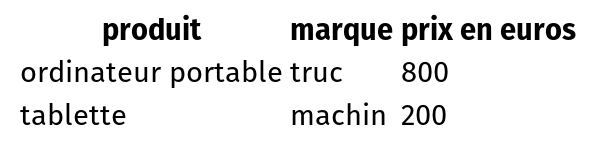
\includegraphics[width=\textwidth, height=0.8\textheight, keepaspectratio]{pics/html_firefox.png}
        \caption{Représentation du code précédent dans un navigateur}
    \end{figure}
    \vskip0pt plus 1fill
    {\tiny Représentation standard dans Mozilla Firefox \shorturl{www.mozilla.org/firefox/}}
\end{frame}

% ██████  ███████ ███████ ███████  ██████  ██    ██ ██████   ██████ ███████ ███████
% ██   ██ ██      ██      ██      ██    ██ ██    ██ ██   ██ ██      ██      ██
% ██████  █████   ███████ ███████ ██    ██ ██    ██ ██████  ██      █████   ███████
% ██   ██ ██           ██      ██ ██    ██ ██    ██ ██   ██ ██      ██           ██
% ██   ██ ███████ ███████ ███████  ██████   ██████  ██   ██  ██████ ███████ ███████


\subsection{Ressources}
\begin{frame}{Les ressources}
    \begin{quote}
        {\only<2>{\small}Toute donnée ou programme disponible pendant l'exécution d'un programme peut être qualifiée de \emph{ressource}.}
    \end{quote}
        \only<2>{
            \begin{itemize}
                \item Listes
                    \begin{itemize}
                        \item[→] mots, caractères…
                    \end{itemize}
                \item Corpus
                \item Bases de connaissances
                    \begin{itemize}
                        \item[→] bases de données, ontologies, lexiques, wordnets…
                    \end{itemize}
                \item Programmes de pré-traitement
                    \begin{itemize}
                        \item[→] segmentation, normalisation…
                    \end{itemize}
                \item Programmes réalisant des traitements linguistiques poussés
                    \begin{itemize}
                        \item[→] lemmatisation, étiquetage morphosyntaxique…
                    \end{itemize}
            \end{itemize}
        }
\end{frame}

\begin{frame}{Quelques ressources linguistiques}
    \begin{itemize}
        \item Le Lexique Extensionnel des Formes Fléchies du Français (Lefff)
            \begin{itemize}
                \item[→] \shorturl[http]{almanach.inria.fr/~sagot/lefff.html}
            \end{itemize}
        \item Wikidata \only<2>{(base de connaissances structurée)}
            \begin{itemize}
                \item[→] \shorturl{www.wikidata.org}
            \end{itemize}
        \item UDPipe \only<2>{(programme)}
            \begin{itemize}
                \item[→] \shorturl{ufal.mff.cuni.cz/udpipe}
            \end{itemize}
        \item Le \alt<1>{French Treebank}{corpus arboré pour le français (French Treebank)}
            \begin{itemize}
                \item[→] \shorturl[http]{ftb.linguist.univ-paris-diderot.fr}
            \end{itemize}
        \item Universal dependencies \only<2>{(ensemble de corpus)}
            \begin{itemize}
                 \item[→] \shorturl{universaldependencies.org}
            \end{itemize}
        \item JeuxDeMots \only<2>{(réseau lexical)}
            \begin{itemize}
                \item[→] \shorturl{www.jeuxdemots.org/jdm-about.php}
            \end{itemize}
    \end{itemize}
    \only<1>{De quelle type de ressource s'agit-il ?}
\end{frame}

% ██████  ██████   ██████   ██████  ██████   █████  ███    ███ ███    ███ ███████ ███████
% ██   ██ ██   ██ ██    ██ ██       ██   ██ ██   ██ ████  ████ ████  ████ ██      ██
% ██████  ██████  ██    ██ ██   ███ ██████  ███████ ██ ████ ██ ██ ████ ██ █████   ███████
% ██      ██   ██ ██    ██ ██    ██ ██   ██ ██   ██ ██  ██  ██ ██  ██  ██ ██           ██
% ██      ██   ██  ██████   ██████  ██   ██ ██   ██ ██      ██ ██      ██ ███████ ███████


\subsection{Programmes}
\begin{frame}{Programmes}
    Première option : programmes « écrits à la main »
    \begin{itemize}
        \item Reposent sur des \alert{connaissances expertes}
        \item Adaptés dans des contextes \alert{stables} et \alert{non-adverses}
        \item Peu de robustesse aux changements et à l'\alert{hétérogénéité}
        \item Dans un contexte adverse (e.g.\ spam vs.\ anti-spam), gare à la course de la reine rouge !
    \end{itemize}
    Attention : ça ne signifie pas que c'est une impasse !
    \begin{itemize}
        \item[→] FRMG (\shorturl[http]{alpage.inria.fr/frmgwiki})
    \end{itemize}
\end{frame}

\begin{frame}{Programmes}
    Deuxième option : \alert{apprentissage artificiel}

    \begin{itemize}
        \item[→] Plutôt que d'écrire des traitements nous-même, on va essayer de les faire générer par la machine
    \end{itemize}

    Hypothèse\footnote{Pas tout à fait vraie} : les humains apprennent à réaliser une tâche en  regardant des \alert{exemples} et en \alert{extrapolant}.

    \begin{itemize}
        \item[→] Donc si on jette suffisamment d'exemples sur un programme qui simule l'apprentissage humain on devrait pouvoir récupérer un programme sans avoir à l'écrire explicitement
    \end{itemize}
\end{frame}

\begin{frame}[fragile]{Programmes}
    \begin{figure}
        \tikzset{external/export=true}
        \begin{tikzpicture}[scale=0.9, every node/.style={transform shape}]
            \node[data] (in) {Entrée};
            \node[program, highlight=a, right=.75cm of in, text width=10ex] (prog) {Programme réalisant la tâche};
            \node[data, right=.75cm of prog] (out) {Résultat};
            \node[program, highlight=6, above=1cm of prog, text width=13ex] (progapp) {Programme d'apprentissage};
            \node[data, highlight=3, right=.75cm of progapp] (mod) {Modèle};
            \node[data, highlight=7, left=.75cm of progapp] (train) {Exemples};
            \draw[->] (in) -- (prog);
            \draw[->] (prog) -- (out);
            \draw[->] (mod) |- ($(prog.north)+(0, 0.5cm)$) -| (prog.north);
            \draw[->] (train) -- (progapp);
            \draw[->] (progapp) -- (mod);
        \end{tikzpicture}
        \caption{Schéma d'une approche par apprentissage artificiel}
    \end{figure}
    Ici le \textcolor{highlighta}{programme réalisant la tâche} est générique, mais utilise comme ressource un \textcolor{highlight3}{modèle} généré par un \textcolor{highlight6}{programme d'entraînement} à partir d'\textcolor{highlight7}{exemples} produits par des humains.
\end{frame}

\begin{frame}{Apprentissage artificiel}
    Avantages
    \begin{itemize}
        \item Peut utiliser des données d'apprentissage génériques
            \begin{itemize}
                \item[→] Permet de concentrer les besoins en connaissances expertes
            \end{itemize}
        \item En général plus \alert{robustes} aux données irrégulières et à l'hétérogénéité
        \item Plus facilement \alert{transférable} (e.g.\ d'une langue à une autre)
    \end{itemize}
    Inconvénients
    \begin{itemize}
        \item Parfois trop peu \alert{explicite}, surtout en \textit{Deep Learning} (mais voir \shorturl{blackboxnlp.github.io})
        \item Dépend beaucoup de la qualité des données d'entraînement
    \end{itemize}
\end{frame}

\begin{frame}{Quelques exemples}
    Quelques exemples de programmes issus d'apprentissage automatique
    \begin{itemize}
        \item SEM (POS tagging, chunking, détection d'entités nommées)
            \begin{itemize}
                \item[→] \shorturl{apps.lattice.cnrs.fr/sem}
            \end{itemize}
        \item UDPipe (segmenteur/étiqueteur/parser)
            \begin{itemize}
                \item[→] \shorturl{ufal.mff.cuni.cz/udpipe}
            \end{itemize}
        \item Google translate (traduction)
            \begin{itemize}
                \item[→] \shorturl{translate.google.com}
            \end{itemize}
        \item HMTL (multi-tâches de compréhension)
            \begin{itemize}
                \item[→] \shorturl{huggingface.co/hmtl/}
            \end{itemize}
        \item @picdescbot (description d'images en langage naturel\footnote{Encore plus fort : \citetitle{alishahi2017encoding} \parencite{alishahi2017encoding}}
            \begin{itemize}
                \item[→] \shorturl{twitter.com/picdescbot}
            \end{itemize}
    \end{itemize}
\end{frame}

%  █████  ██████  ██████  ███████ ███    ██ ██████  ██ ██   ██
% ██   ██ ██   ██ ██   ██ ██      ████   ██ ██   ██ ██  ██ ██
% ███████ ██████  ██████  █████   ██ ██  ██ ██   ██ ██   ███
% ██   ██ ██      ██      ██      ██  ██ ██ ██   ██ ██  ██ ██
% ██   ██ ██      ██      ███████ ██   ████ ██████  ██ ██   ██

\appendix
\pgfkeys{/metropolis/inner/sectionpage=simple}  % Avoid random errors with section page progressbar
\section{Annexes}
\pdfbookmark[2]{Remerciements}{acknowledgements}
\begin{frame}{Remerciements}
    Ce cours a été construit à partir du polycopié de cours \citetitle{tellier2017fouille} \parencite{tellier2017fouille} et des précieux conseils d'Isabelle Tellier que je ne saurais trop remercier pour sa confiance et son dévouement.
\end{frame}

\pdfbookmark[2]{Références}{references}
\begin{frame}[allowframebreaks]{References}
    \printbibliography[heading=none]
\end{frame}

\pdfbookmark[2]{Licence}{licence}
\begin{frame}{Licence}
    \begin{center}
        {\huge \ccby}
        \vfill
        This document is available under the terms of the Creative Commons Attribution 4.0 International License (CC BY 4.0) (\shorturl{creativecommons.org/licenses/by/4.0})

        Exceptions to the above statement are listed at {\small\shorturl{loicgrobol.github.io/intro-fouille-textes\#licences}}
        \vfill
        © 2019, Loïc Grobol <\shorturl[mailto][:]{loic.grobol@gmail.com}>

        \shorturl[http]{lattice.cnrs.fr/Grobol-Loic}
    \end{center}
\end{frame}

\end{document}
